\chapter{Introduction}

\section{Background}
Stethoscopes reveal vital diagnostic information about a patient's heart, lungs and airways\cite{Grais2013}. At the Royal Melbourne Hospital patients with infectious and potentially fatal diseases, like Ebola, are going to be treated in isolation rooms. These rooms are specially designed so that diseases can not get out, preventing any potential outbreak. Doctors in these rooms would like to be able to use a stethoscope to aid diagnosis,however they can't use a conventional stethoscope because they need to wear full body protection suits. These suits are equipped with fans to keep the interior at positive pressure, which keeps diseases outside of the suits and protects the occupant from infection. 

Current commercially available electronic stethoscopes require the user to wear Blue tooth ear pieces. These are not feasible for use in the isolation room as the doctors can not adjust the ear pieces with the suit on. Also when doctors take off their isolation suites they want to minimise the chance of touching their face after removing the helmet but while they're still wearing the body piece. This could potentially act as a disease vector from the suit to the practitioner, and is more likely to happen if they are using an ear piece which they would instinctively want to take off after removing the helmet. Furthermore the price of the commercially available electronic stethoscopes is approximately \$800, which is prohibitively expensive. This is because the doctors need to discard the stethoscope after use on a single patient as it is contaminated with an infectious disease. Thus a new wireless stethoscope must be developed to be used in these isolation rooms.

\section{Project Aims}
This project aims to modify a new cheaper stethoscope that uses electronic sensors to detect and transmit sound data to a speaker interface. This electronic stethoscope (Fig.~\ref{fig:design_idea}) will be designed for use in isolation rooms at Royal Melbourne Hospital, enabling doctors to perform auscultations without compromising the integrity of their isolation suits. 

\begin{figure}[!htbp]
	\centering
		\fbox{
		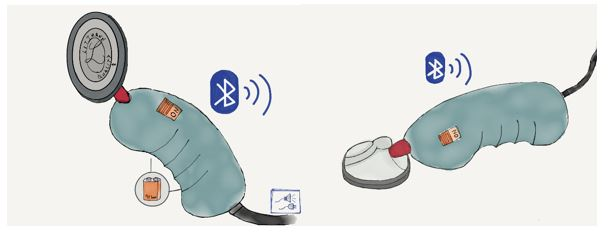
\includegraphics[width=140mm]{design_idea.jpg}
		}
	\caption{Idea to modify conventional stethoscope for wireless sound transmission}
	\label{fig:design_idea}
\end{figure}

\subsection{Product Requirements}
The stethoscope must not compromise the isolation suites used in the isolation room. The design should have a diaphragm that operate like a traditional stethoscope so that the doctors are familiar with the product and it does not change the behaviour of doctor using traditional stethoscope. The sound signal should be adjustable and output via a wired speaker and wireless speaker.  Besides, the electronic stethoscope can be powered by a battery or external wall adapter. And the battery must last life time of a single patient. The size of the product should be small enough so that it can be held by a single hand. At last, the cost of the product should be cheaper than the current available electronic stethoscope.

\subsection{Product Specification}
\subsubsection{Sound Signal collection}
Sound Signal is collected by using a conventional diaphragm (Fig.~\ref{fig:conventional_stethoscope}). A traditional stethoscope can be easier to modify to a wireless stethoscope by attach the diaphragm to the product.
\begin{figure}[!htbp]
	\centering
		\fbox{
		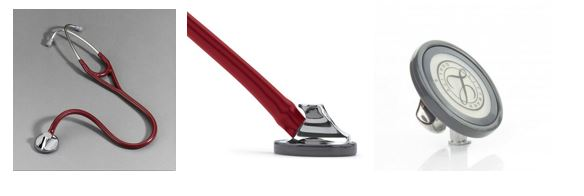
\includegraphics[width=140mm]{conventional_stethoscope.jpg}
		}
	\caption{Conventional stethoscope}
	\label{fig:conventional_stethoscope}
\end{figure}

\subsubsection{Signal processing}
Micro-controller is included in the design in order to do digital signal processing. Removing noise, cancelling feedback and other signal processing may be required when the product operates in different environments. Digital Signal Processing is more flexible than in physical signal processing

\subsubsection{Size}
The electronic board is approximately 15cm length and 5 cm wide and covered by a plastic cylinder. A cone or a short part of tube is provided to connect the diaphragm and the plastic cylinder 
 
\subsubsection{Power supply}
Two different power supply options are provided.
A battery or rechargeable battery makes it more portable.
External wall plug-in adapter makes it last long time operation.

\subsubsection{Output format}
Sound signal form diaphragm can be played through a wired speaker and a Blue tooth speaker.
Volume can be adjustable.

\subsubsection{Indication}
There are different LEDs to indicate different operation stages, such as power on, Blue tooth operation and so on.

\subsubsection{Cost}
The total cost of product to modify the conventional stethoscope is lower than the half price of the current available wireless stethoscope since the stethoscope may be modified to use for training purpose.
